%...import de package...
\documentclass[12pt]{article}
\usepackage[utf8]{inputenc}
\usepackage[a4paper]{geometry}
\usepackage[myheadings]{fullpage}
\usepackage{fancyhdr}
\usepackage{lastpage}
\usepackage{wrapfig, subcaption, setspace, booktabs}
\usepackage[T1]{fontenc}
\usepackage[font=small, labelfont=bf]{caption}
\usepackage{fourier}
\usepackage[protrusion=true, expansion=true]{microtype}
\usepackage[francais]{babel}
\usepackage{sectsty}
\usepackage{url, lipsum}
\usepackage{tgbonum}
\usepackage{hyperref}
\usepackage{xcolor}
\usepackage{graphicx}
\usepackage[none]{hyphenat}
\usepackage{endnotes}
\usepackage{multirow}
\usepackage{epstopdf}
\usepackage[export]{adjustbox}
\renewcommand{\footnote}[1]{\endnote{#1}}
\renewcommand{\theendnote}{}


\newcommand{\HRule}[1]{\rule{\linewidth}{#1}}
\onehalfspacing
\setcounter{tocdepth}{5}
\setcounter{secnumdepth}{5}


%...page de couverture...
\begin{document}
\begin{figure}[t]
	\includegraphics[width=4cm]{logo_esiee.jpeg}
\end{figure}

\fontfamily{cmr} \selectfont
\title{ \normalsize \textsc{}
	\\ [2.0cm]
	\HRule{0.5pt} \\
	\LARGE \textbf{\uppercase{Rapport de projet ITW}
	\HRule{2pt} \\ [0.5cm]
	\normalsize  \vspace*{5\baselineskip}}
}

\author{Théo PERESSE-GOURBIL et Manon HERMANN}
\date{Octobre-Novembre 2019}
\maketitle
\newpage

%...page d'intro...
\section{Introduction}
    %présenter le sujet, ce qu'on va y faire (etc)
Dans le cadre de nos études, nous avons dû développer un site internet à destination du monde étudiant.
C'est dans la matière ITW \textit{(introduction aux technologies du web)} que ce mini-projet est mis en place.
\\
Le site doit être statique et non-responsive. Il doit comporter plusieurs pages, notamment :
\begin{itemize}
    \item page d'accueil,
    \item page actualité,
    \item page logement,
    \item page voyage,
    \item page réseaux sociaux,
    \item page contact,
    \item page mention légale
\end{itemize}

\vspace{1\baselineskip}

Nous avons choisi de faire notre page sur un sujet "sur-réaliste" : un monde étudiant inter-galactique en immersion dans le monde de \textit{Star Wars Story}.
C'est-à-dire qu'il existerait plusieurs planètes habitables dans différents systèmes galactiques, où chaque planète à une spécialité d'étude.\\


Les actualités comprennent des évènements présents sur les planètes, des informations géopolitiques, de nouvelles formations disponibles\ldots

Les logements proposés vous permettent d'observer l'architecture de chaque planète, leur prix, les types de séjours que vous pourrez réserver\ldots

Les offres de voyages montrent les exclusivités, les activités\ldots \\


Ce site web est bien évidemment factice et nous avons dû respecter plusieurs consignes concernant l'aspect global des pages, les technologies utilisés, le contenu \ldots
\newpage

%...table des matières...
\tableofcontents
 \vspace{4\baselineskip}
\newpage


%...début du rapport...
\sectionfont{\scshape}

\section{Arborescence}
    %arborescence du site internet (quel page est relier avec laquelle...)
L'arborescence de notre site web est telle que nous pouvons accéder à chacune des pages grâce au menu du haut de page ("accueil", "actualités", "logements", "voyages") et le menu du bas de page ("mention légale", "contact", "réseaux sociaux").

\begin{figure}[h]
    \centering
    \includegraphics[scale=0.5]{arbo.png}
\end{figure}

Sans utiliser ces menus, il est possible depuis la page d'"accueil" d'être dirigé sur les pages "actualités", "logements" ou "voyages".
Depuis la page "mention légale" on peut accéder à celle des "réseaux sociaux", dans laquelle on peut aller sur le projet Git (pour télécharger les sources et le code LaTeX) et la page Facebook du projet. 


\newpage
\section{Zoning}
    % le design de chaque page
Le design de chaque page a été faite selon les critères donnés par le responsable de l'unité. Il fallait donc reprendre le zoning de page déjà existante :
\begin{itemize}
    \item "Accueil" : https://www.louvre.fr/
    \item "Actualité" : https://www.lesechos.fr/
    \item "Logement" : https://www.seloger.com/
    \item "Voyage" : https://sejour.govoyages.com/
\end{itemize}
\vspace{2\baselineskip}


\begin{minipage}{0.5 \linewidth}
    \hspace{-3cm}
    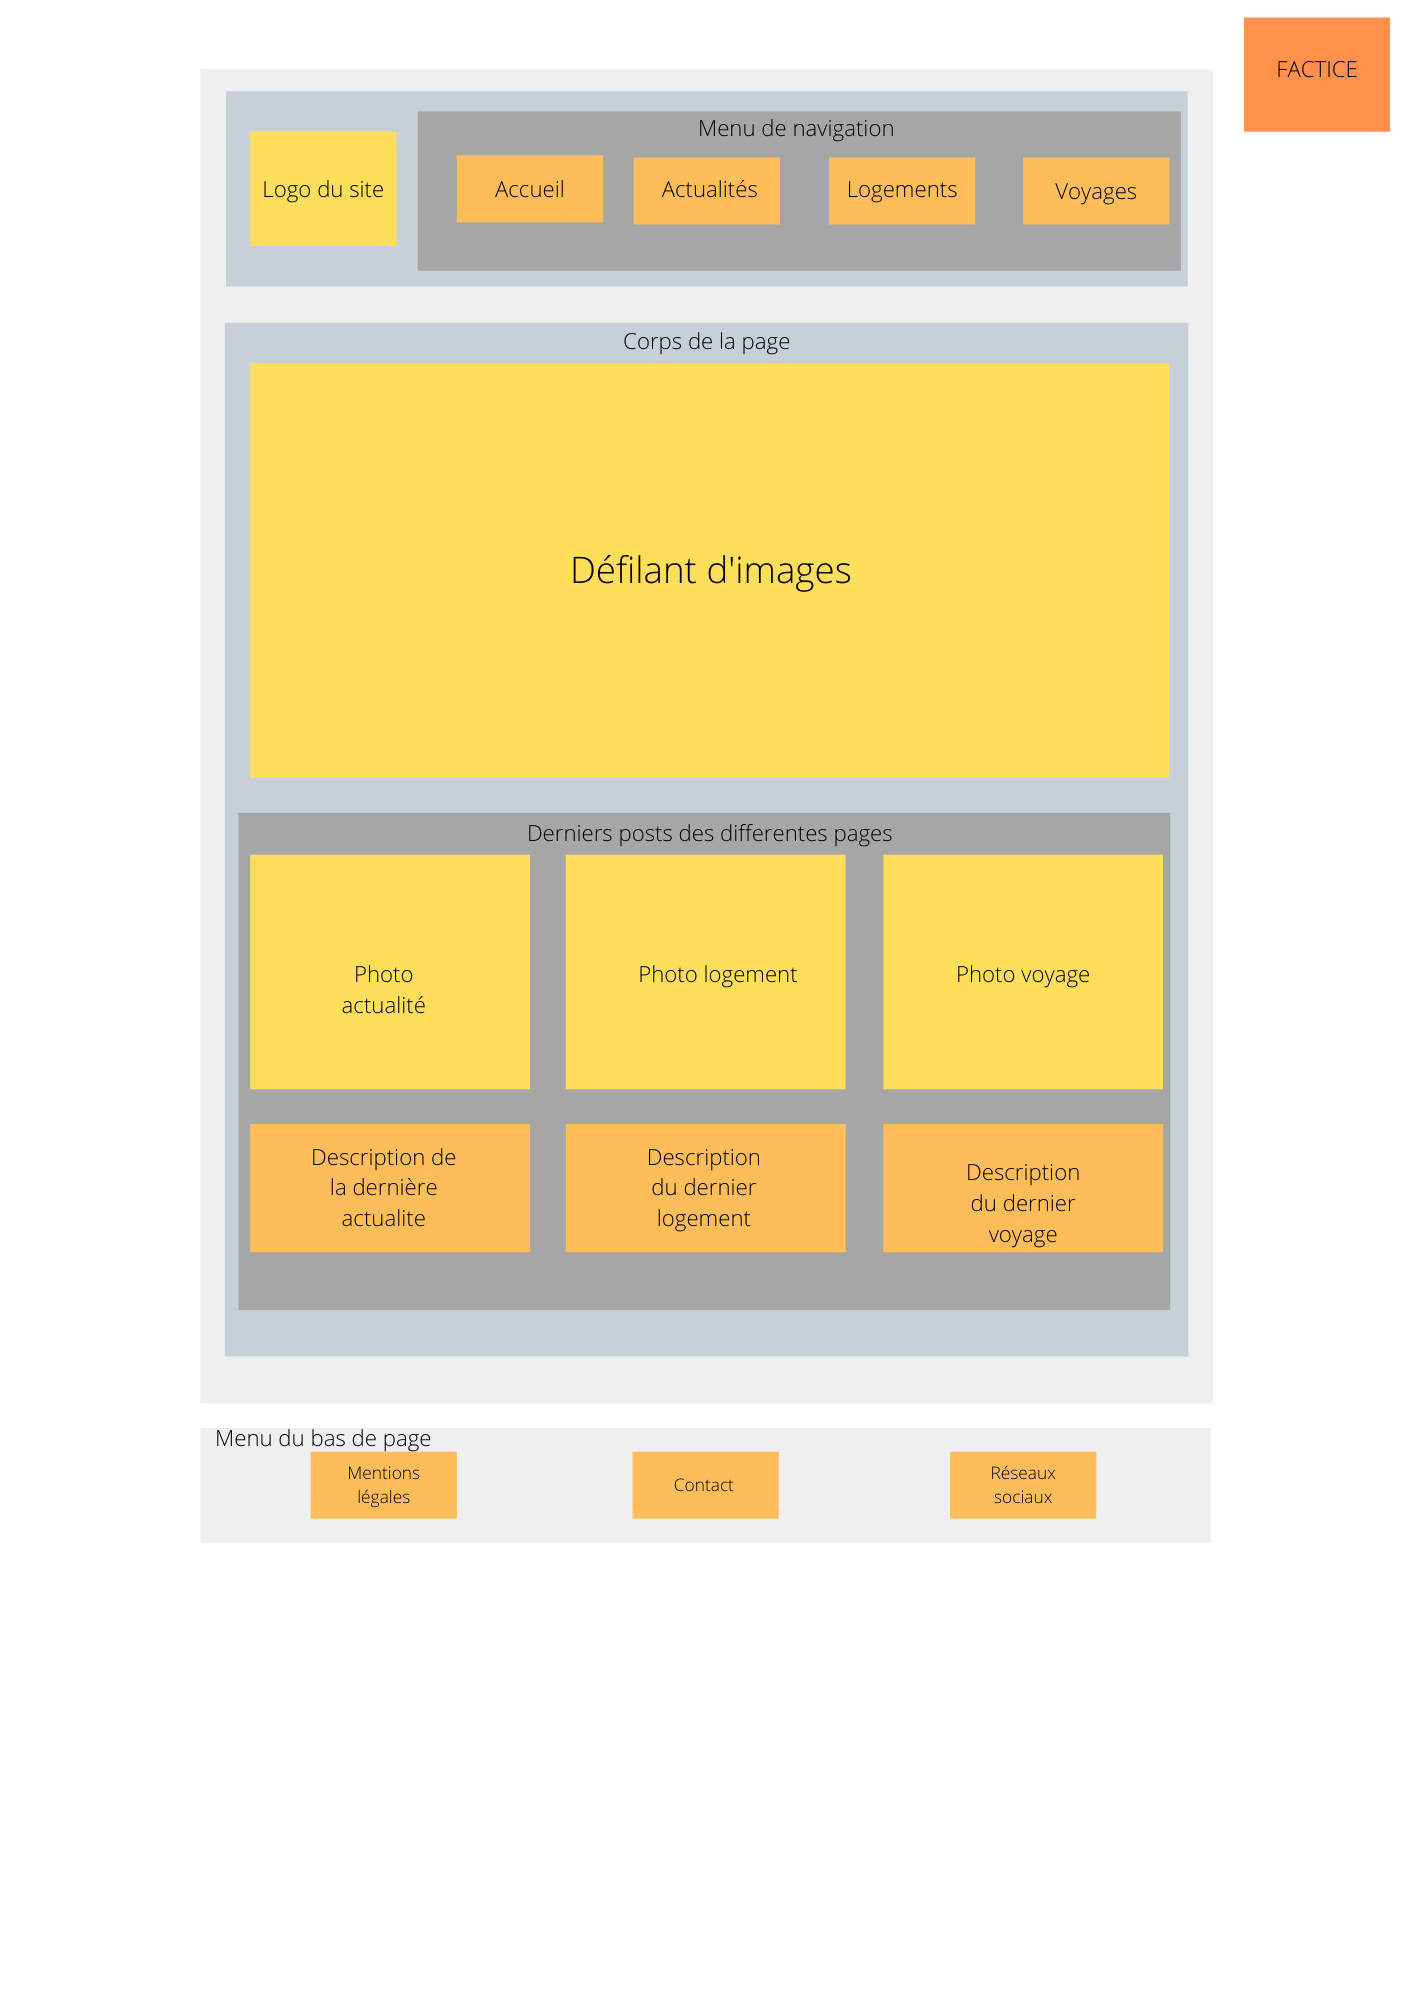
\includegraphics[scale=0.3]{accueil.png}
\end{minipage} \hfill
\begin{minipage}{0.5 \linewidth}
    Cette page "accueil" contient le menu en haut de page qui est commun avec les autres pages, ainsi que le pied de page, lui aussi commun avec l'intégralité des pages du projet. 
    On retrouve aussi un défilant de 4 images dans la partie supérieure du corps de la page. 
    En dessus, 3 actualités en lien avec les différentes pages sont composées d'une description et d'une image.
\end{minipage}

\begin{minipage}{0.5 \linewidth}
   Cette page "actualité" contient, comme précédemment, le menu en haut de page et le bas de page. 
   Elle a sa dernière actualité en plus grande pour la mettre en avant : iframe d'une carte intergalactique avec la description de l'actualité. 
   Deux autres sont ajoutées à la suite, les images sont plus petites et les descriptions plus concises.
\end{minipage} \hfill
\begin{minipage}{0.5 \linewidth}
    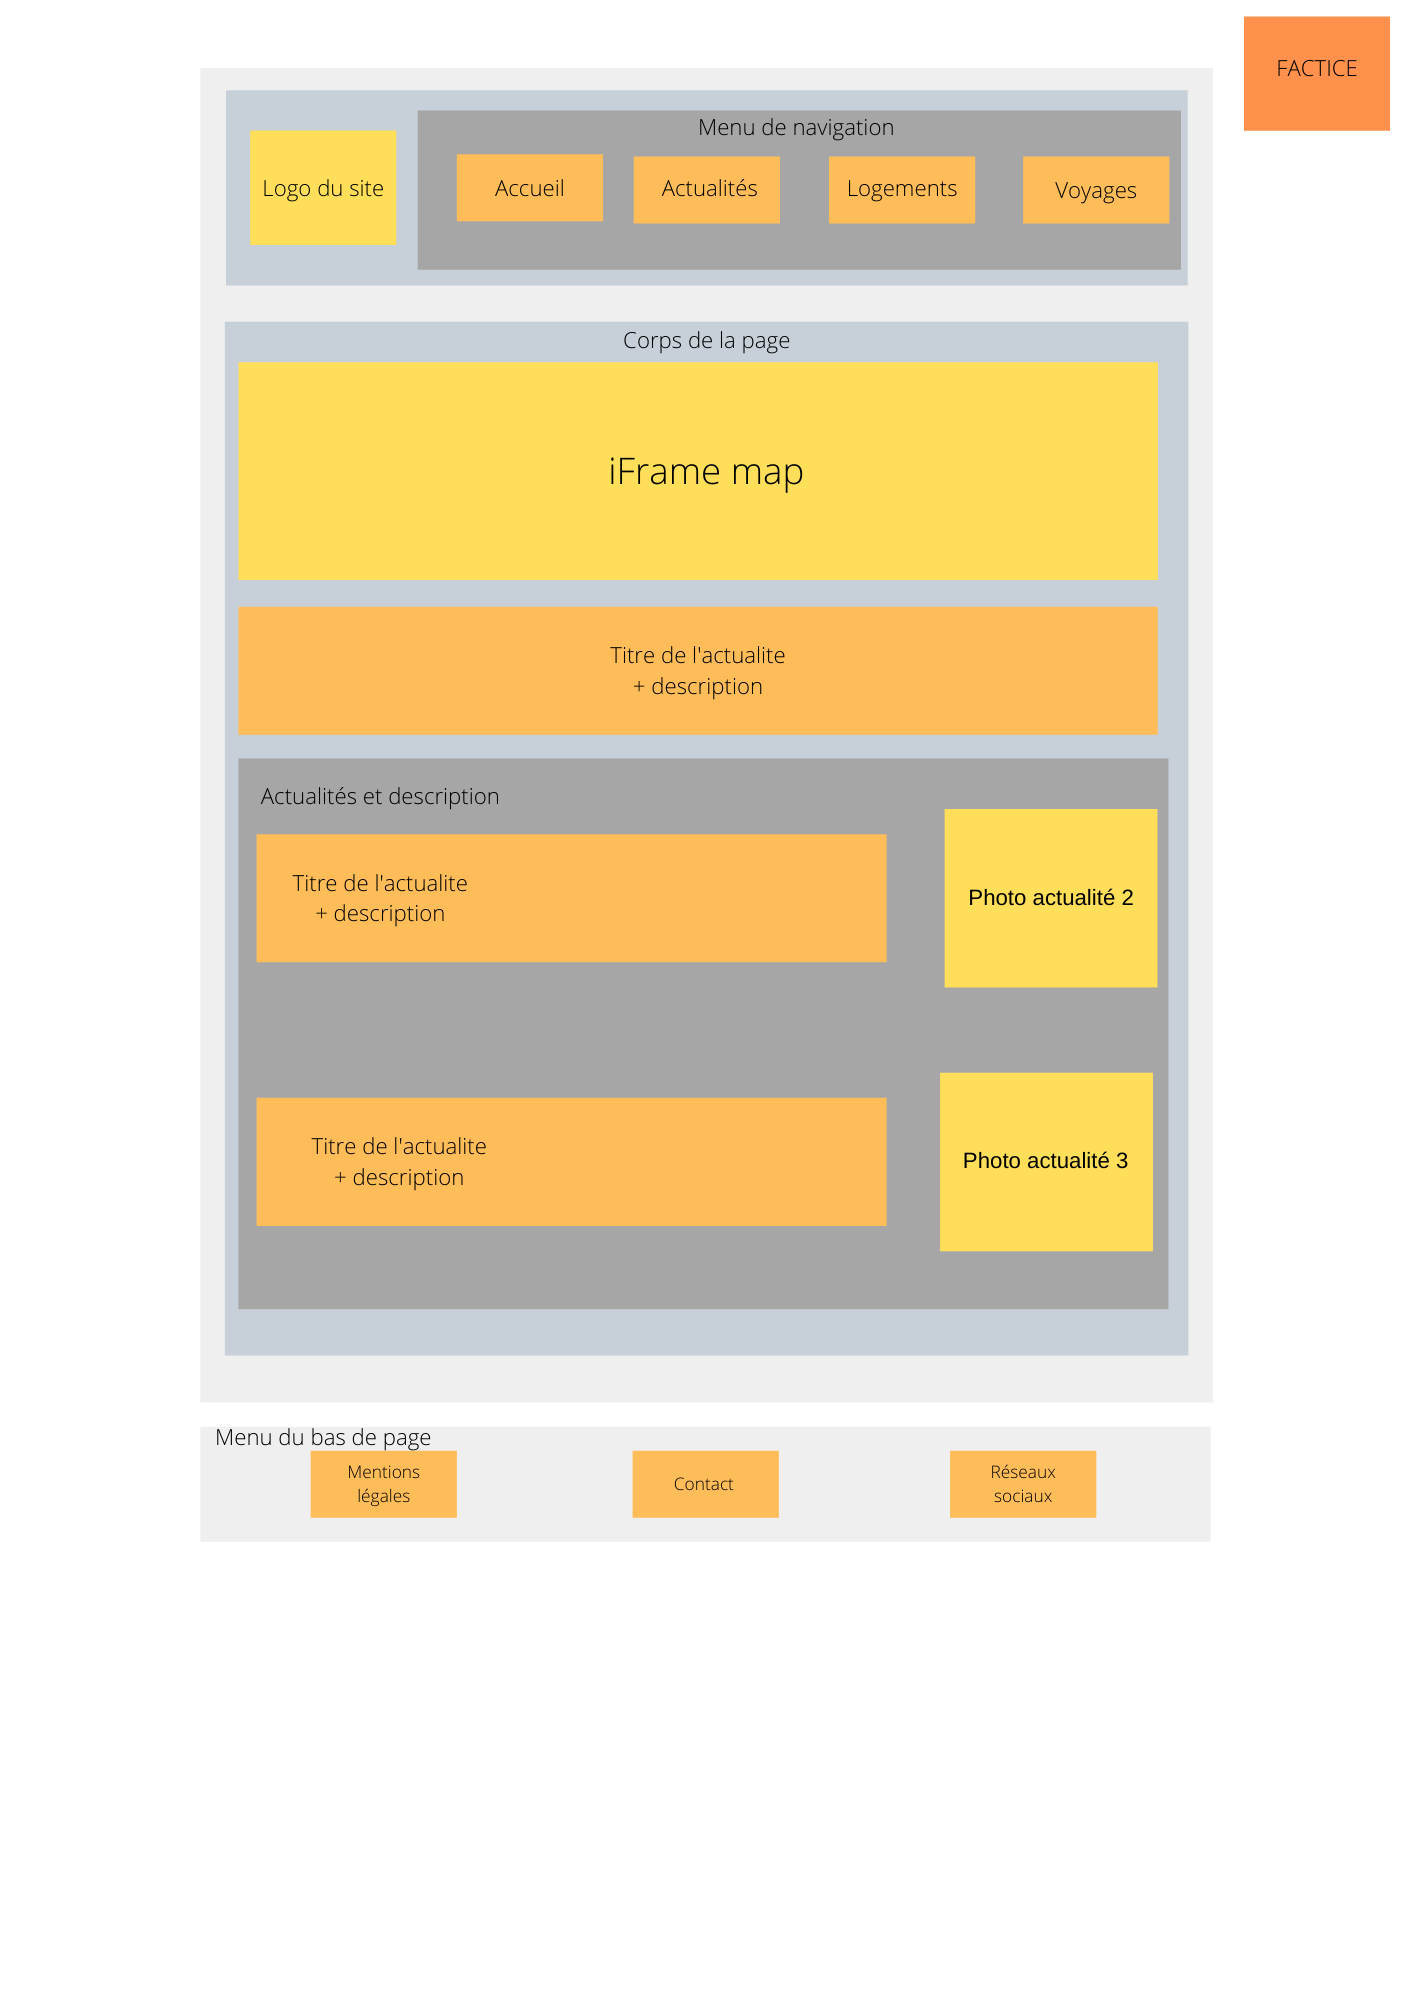
\includegraphics[scale=0.21]{actualite.png}
\end{minipage}

\begin{minipage}{0.5 \linewidth}
    \hspace{-1cm}
    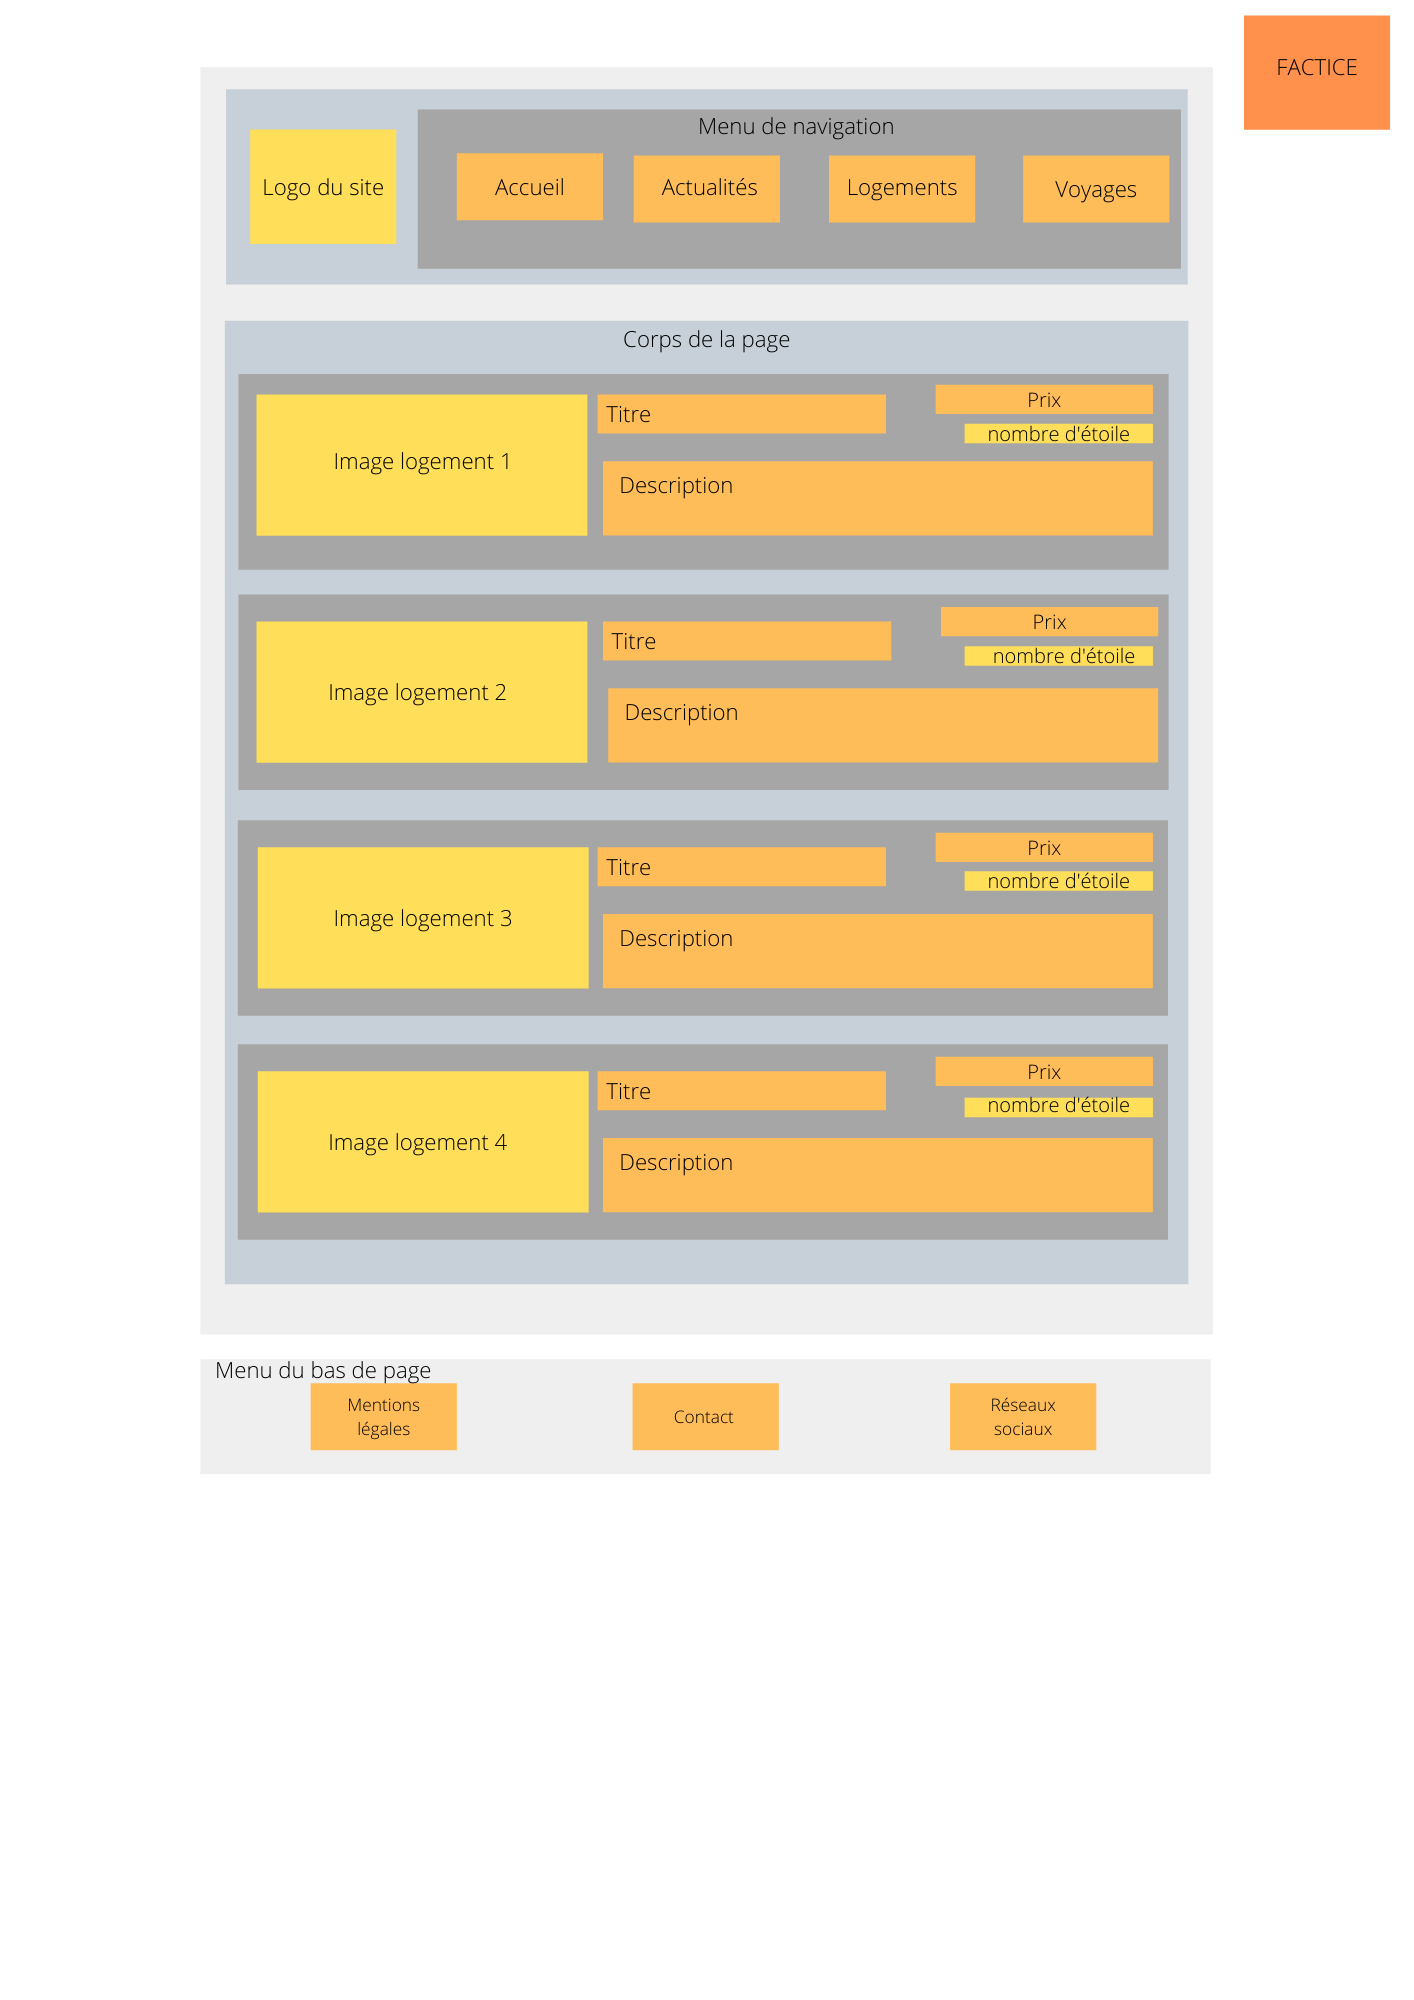
\includegraphics[scale=0.21]{logement.png}
\end{minipage} \hfill
\begin{minipage}{0.5 \linewidth}
    De même pour la page "logement", le menu en haut et bas de page sont disponibles.
    Ici, il y a quatre types de logement possible. 
    Ils sont tous implémenté de la même façon : image d'illustration à gauche, le titre du voyage et sa description, le prix ainsi que la note attribuée au logement par les précèdent clients.
\end{minipage}

\begin{minipage}{0.3 \linewidth}
    Pour finir, la page "voyage" a elle aussi les menus du haut et du bas de page.
    La structure est différentes pour celle-ci : il y a six voyages disponibles.
    Ils sont organisés sur deux lignes.
    Chacun à une image, un titre et une description ainsi qu'un prix.
\end{minipage} \hfill
\begin{minipage}{0.5 \linewidth}
    \hspace{-2cm}
    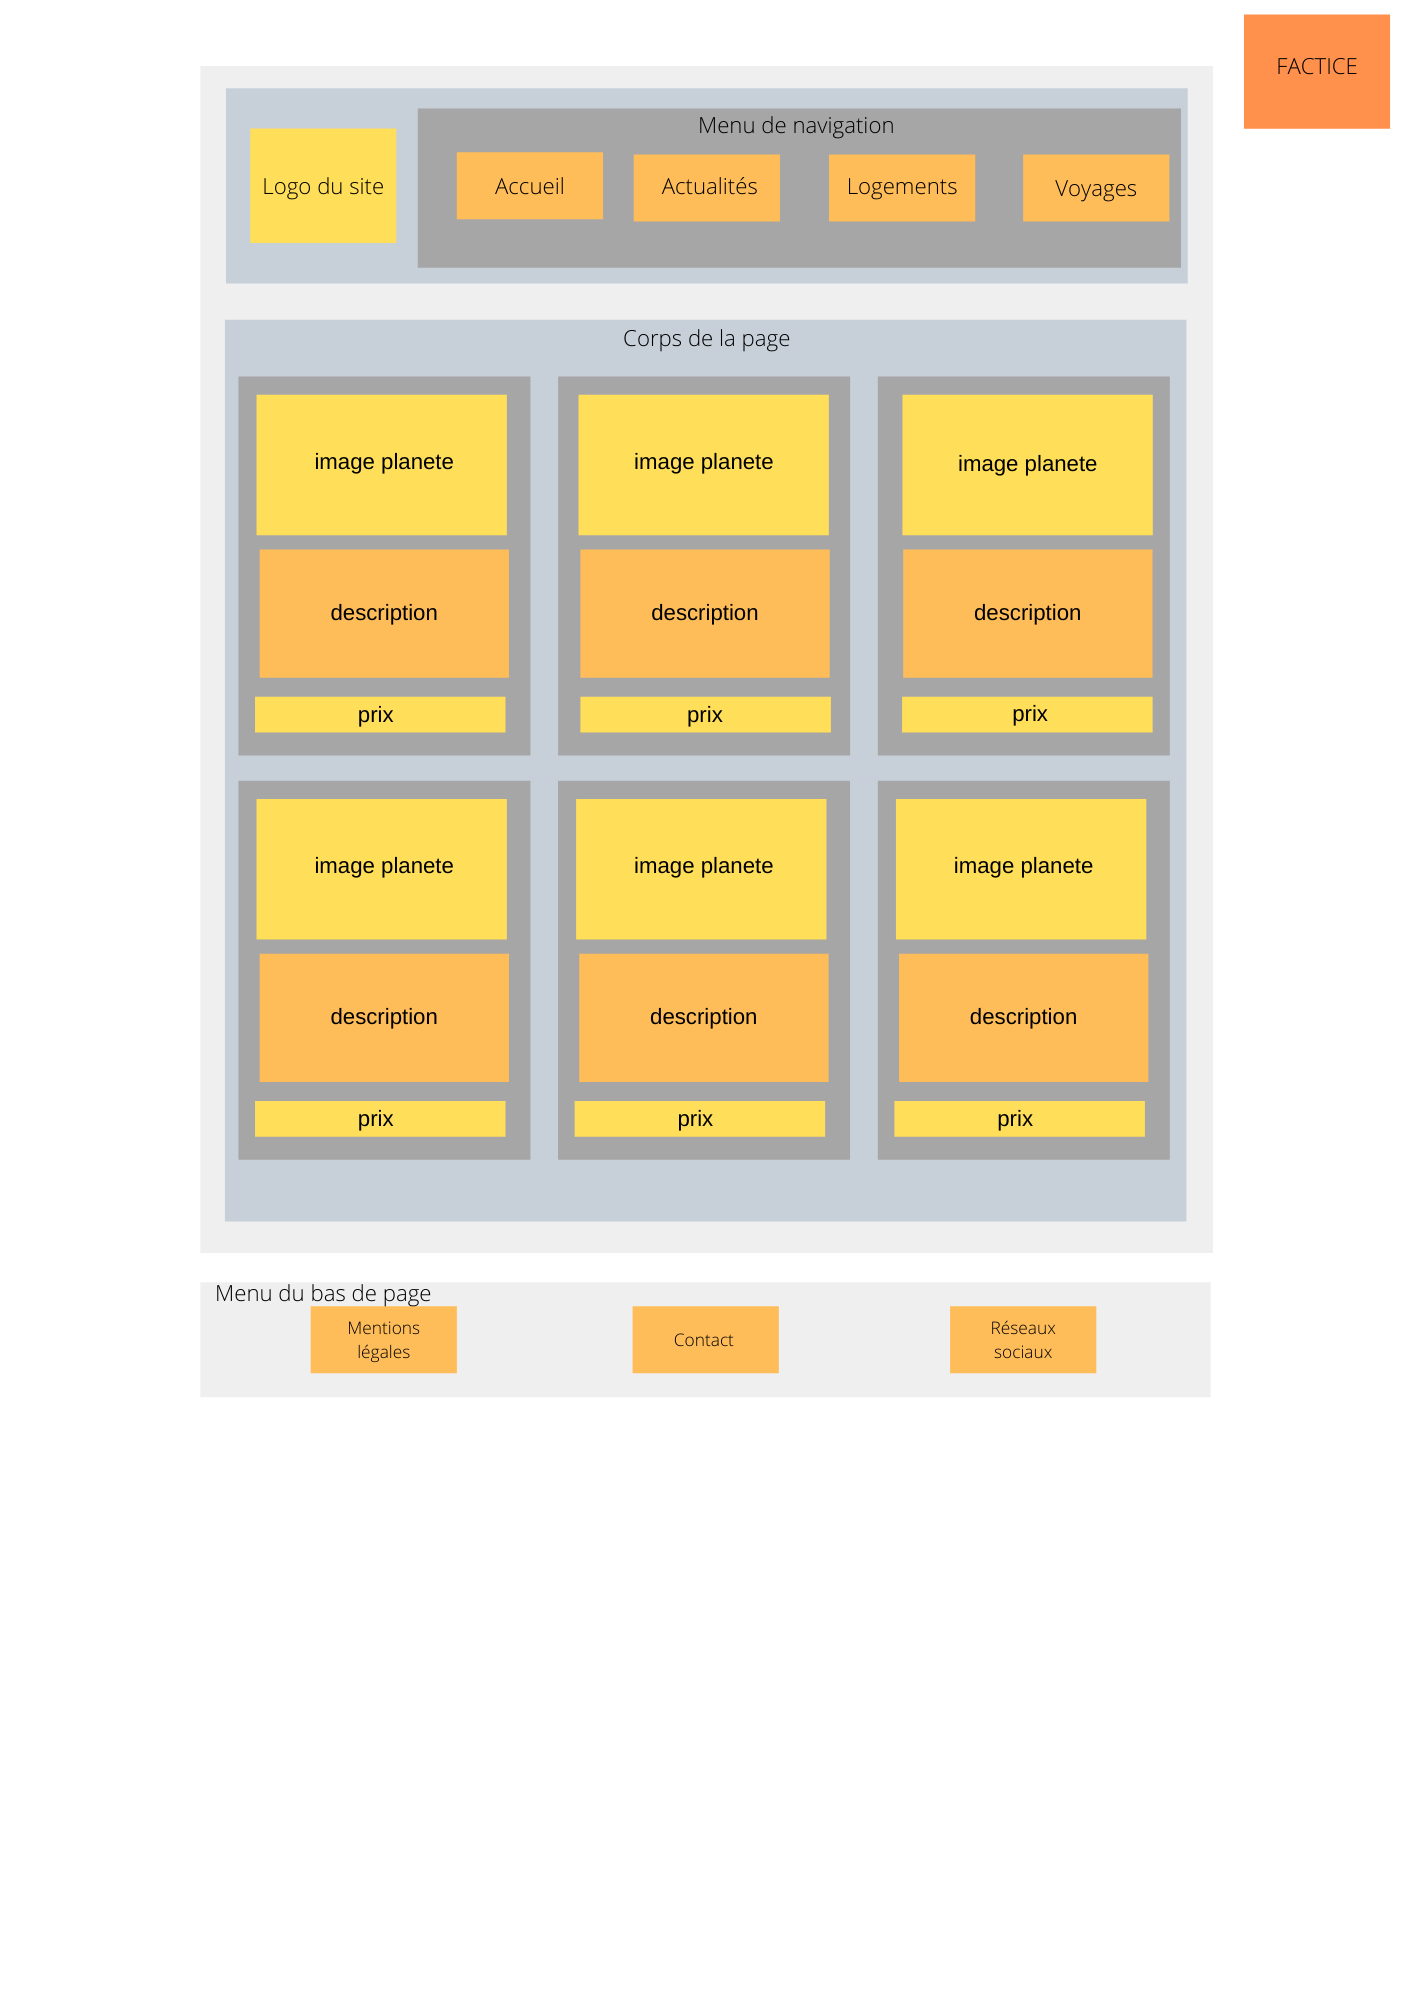
\includegraphics[scale=0.3]{voyage.png}
\end{minipage}

Sur les pages "logements" et "voyages", nous avons implémenté un tableau de conversion des monnaies galactiques. 
Celui-ci peut disparaître hors de la page ou apparaître sur le côté par le simple survole des flèches à cet effet.

Les pages "mention légale", "contact", "réseaux sociaux" n'ont pas été faite sur un modèle. 
Les groupes étaient libres pour le zooning de celles-ci. 

\newpage
\newpage
\section{Organisation}
    %répartition et organisation du travail au sein des semaines de projet
Nous avons décidé de travailler bien évidement lors des séances, mais aussi en dehors des séances du vendredi pour avancer au mieux et régulièrement notre projet.\\

Le travail est partagé dans sa totalité et chacun de nous avons contribué à chaque technologie (HTML, CSS, JavaScript, LaTeX, Git\ldots).
Nous avons tout d'abord pris beaucoup de temps pour discuter autour du sujet, de l'aspect, du zoning des pages pour ensuite nous faciliter l'avancement du site web.
Pour pouvoir travailler chacun de notre côté, nous avons basé notre projet sur GitHub, nous permettant ainsi d'y contribuer simultanément. \\

Concernant la répartition du travail sur les différentes semaines, nous avons décidé de : 
\begin{itemize}
    \item Commencer par l'aspect commun de toutes les pages, 
    \item Concevoir la page d'accueil, 
    \item Rassembler nos idées pour les différentes sections dans les actualités, les logements et les voyages,
    \item Concevoir les 3 pages HTML séparément.
\end{itemize}
De plus, ce rapport de projet a été avancé majoritairement au début du projet (introduction, technologie utilisées, organisation).
Mais nous avons surtout voulu compléter au fur et à mesure d'autres sections comme le reporting du temps passé, les problèmes et bugs rencontrés, et peaufiner le CSS afin d'avoir un rendu qui nous plaît mais aussi ajouter des fonctionnalités optionnels notamment des scripts JavaScript. 


\newpage
\section{Technologie utilisé}
    %détail des technologies employées / plugins utilisés
Concernant les technologies utilisées, nous avons voulu utiliser le plus de technologie possible afin de monter en compétence durant ce projet dans différentes technos. C'est pourquoi nous avons utilisés les outils suivants : 
\begin{itemize}
    \item HTML, pour la structure de la page ;
    \item CSS, pour le design de celle-ci ;
    \item JavaScript, pour le comportement des pages ;
    \item Le protocole Git et le client GitHub pour le versionnement du code ;
    \item LaTeX et Overleaf pour la réalisation de ce dossier ;
    \item Gimp pour le traitement d'image.
\end{itemize}
\vspace{1\baselineskip}

Chaque page à son propre fichier HTML (1 pour l'accueil, 1 pour les actualités, 1 pour le logement, 1 pour les voyages). 
Tandis qu'il existe une feuille de style CSS commune à toutes ces pages contenant le fond, le menu de navigation et le bas de page car il est identique pour chacune d'elles. 
Ainsi qu'une page style propre à celles-ci.      \\

Certains scripts ont été ajoutés pour faire les animations sur les pages : \begin{itemize}
    \item Défilant d'images sur la page "accueil" ;
    \item Tableau interactif qui apparaît et disparaît sur les pages "logements" et "voyages" ;
    \item Pop-up lorsqu'on clique sur envoyer le formulaire sur la page "contact".
\end{itemize}


% + les références de nos copier-coller

\newpage
\section{Reporting du temps passé}
    %reporting précis du temps passés par tache
Voici notre reporting de temps passé par jour et par tâche. \\
\textit{Ce temps est approximatif, nous n'avons pas chronométré chacune de nos tâches.} 
\bigbreak

\begin{center}
\begin{tabular}{|c|c|l|}
    \hline
    \textbf{Date} & \textbf{Temps} & \textbf{Description} \\
    
    \hline
     \multirow{2}{*}{18/10} & 15 min & Lecture du sujet \\
            & 45 min & Imagination de notre site web \\
            
    \hline
     \multirow{2}{*}{24/10} & 2 h & Menu de navigation \\
            & 30 min & Recherches  \\
            
    \hline
    \multirow{2}{*}{25/10} & 1 h 30 & Bas de page \\
            & 45 min & Rapport de projet \\
    
    \hline
    26/10 & 3 h & Formulaire contact \\
    
    \hline
    \multirow{3}{*}{17/10} & 1 h 30 & Défilant d'image sur l'accueil \\
        & 1 h & Polices StarJedi \\
        & 30 min & Bugs \\
    
    \hline
    \multirow{3}{*}{29/10} & 30 min & Page mention légale \\
        & 30 min & Modification d'images \\
        & 1 h & Page voyage \\
    
    \hline
    04/11 & 2 h & Page logement html et css \\
    
    \hline
    \multirow{3}{*}{08/11} & 30 min & Mise à jour des images \\
        & 1 h 30 & Page actualité html et css \\
        & 30 min & Modification avec le professeur \\
        
    \hline
    11/11 & 1 h & CSS page actualité \\
    
    \hline
    \multirow{3}{*}{15/11} & 45 min & Modification des descriptions des voyages \\
        & 30 min & Ajout des notes sur le logement \\
        & 1 h & Fenêtre qui apparaît et disparaît (page logement et voyage) \\
        
    \hline
    20/11 & 30 min & Travail sur l'iframe \\
        
    \hline
    \multirow{4}{*}{21/11} & 30 min & Zooning des pages \\
        & 15 min & Modification des images \\
        & 2 h & CSS du tableau des conversions des monnaies \\
        & 30 min & Page Réseaux sociaux \\
        
    \hline
    \multirow{2}{*}{22/11} & 45 min & Fin du rapport \\
        & 30 min & Détails estétique sur le site web \\
        
    \hline
        

\end{tabular}
\end{center}

\newpage
\section{Problèmes et bugs rencontrés}
    %liste des problèmes / bugs rencontrés

Le fait qu'une taille de page (1000 pixels de largeur) nous soit imposée nous a compliqué la tâche.
En effet, tous les ordinateurs n'ayant pas la même résolution, il aurait été plus facile de tout paramétrer (dans le CSS) avec des pourcentages pour que l'affichage s'adapte automatiquement.\\

Un gros problème que nous avons eu, et que nous n'arrivons toujours pas à expliquer (et donc à résoudre), est un souci d'affichage de notre iframe qui devait contenir une carte inter-galactique du monde de Star Wars.
L'erreur est la suivante : \textit{Alternate HTML content should be placed here. This content requires the Adobe Flash Player. Get Flash}.
Le souci étant que sur certains ordinateurs, l'iframe s'affiche correctement, notamment avec le plug-in intégré Firefox, mais uniquement sur certains ordinateurs avec Firefox.

\newpage
\section{Conclusion}
    %faire une conclusion ...
Ce projet fut pour nous l'occasion de découvrir la bibliothèque JavaScript jQuerry et d'améliorer nos compétences en HTML, CSS et JS. De plus, nous avons aussi progressé avec Git, notamment la résolution de merge et de branch. \\



Pour pouvoir observer l'avancement de ce projet au fils du temps, vous avez la possibilité d'aller sur notre projet Git, \url{https://github.com/blackjack-nix/projetITW/commits/master}. \\
De plus, pour télécharger le projet, dans un terminal, tapez : 

git clone https://github.com/blackjack-nix/projetITW/ \\
Ce dossier contient le code du projet, une version compilée du rapport, mais aussi les sources LaTeX afin de recompiler le PDF.
\newpage

\end{document}